\documentclass[10pt,aspectratio=169]{beamer}

% All the boilerplate is in deslides.sty
\usepackage{deslides}

\author{Ji\v{r}\'i Lebl}

\institute[OSU]{%
Oklahoma State University%
%Departemento pri Matematiko de Oklahoma {\^S}tata Universitato%
}

\title{22. Forced oscillations and resonance, \\part 2: Damped forced motion
and practical resonance\\(Notes on Diffy Qs, 2.6)}

\date{}

\begin{document}

\begin{frame}
\titlepage

%\bigskip

\begin{center}
The textbook: \url{https://www.jirka.org/diffyqs/}
\end{center}
\end{frame}

\begin{frame}
Recall our setup:

\medskip

\hfill\scalebox{0.85}{\subimport*{../figures/}{massfigforce.pdf_t}}\hspace*{\fill}

\medskip
\pause

The equation is
\[
mx'' + cx' + kx = F(t) ,
\]
$m$ is the mass,

$c$ if friction,

$k$ is the spring constant, and

$F(t)$ is an external force acting on the mass.

\medskip
\pause

We are considering
\[
F(t) = F_0 \cos (\omega t)
\]
\end{frame}

\begin{frame}
We consider damped ($c > 0$) motion:
\[
mx'' + cx' + kx = F_0 \cos (\omega t) .
\]
\pause
Write:
\vspace*{-9pt}
\[
p = \frac{c}{2m},  \qquad \omega_0 = \sqrt{\frac{k}{m}} .
\]
Equation becomes:
\vspace*{-4pt}
\[
x'' + 2px' + \omega_0^2x = \frac{F_0}{m} \cos (\omega t) .
\]
\pause
Roots of the characteristic equation are
$-p \pm \sqrt{p^2 - \omega_0^2}$, so the complementary solution is
\[
x_c =
\begin{cases}
C_1 e^{r_1 t} + C_2 e^{r_2 t} & \text{if } \; c^2 > 4km , \\
C_1 e^{-p t} + C_2 t e^{-p t} & \text{if } \; c^2 = 4km , \\
e^{-p t} \bigl( C_1 \cos (\omega_1 t) + C_2 \sin (\omega_1 t) \bigr) &
  \text{if } \; c^2 < 4km ,
\end{cases}
\]
where $\omega_1 = \sqrt{\omega_0^2 - p^2}$.

\medskip
\pause

Note that
$x_c(t) \to 0$ as $t \to \infty$.
\end{frame}

\begin{frame}
We need a particular solution.  Try
\[
x_p = A \cos (\omega t) + B \sin (\omega t).
\]
\pause
We plug into the equation $x'' + 2px' + \omega_0^2x = \frac{F_0}{m} \cos
(\omega t)$:
\[
\bigl((\omega_0^2  - \omega^2)B - 2\omega p A\bigr) \sin (\omega t)
+
\bigl((\omega_0^2  - \omega^2)A + 2\omega p B\bigr) \cos (\omega t)
=
\frac{F_0}{m} \cos (\omega t) .
\]
\pause
Solve for $A$ and $B$:
\[
A=\frac{(\omega_0^2-\omega^2) F_0}
{m{(2\omega p)}^2+m{(\omega_0^2-\omega^2)}^2} ,
\qquad
B=\frac{2 \omega p F_0}
{m{(2\omega p)}^2+m{(\omega_0^2-\omega^2)}^2} .
\]
Compute the amplitude of $x_p$:
\[
C = \sqrt{A^2+B^2} = \frac{F_0}{m \sqrt{{(2\omega p)}^2+{(\omega_0^2-\omega^2)}^2}} .
\]
\end{frame}

\begin{frame}
So our particular solution is
\begin{multline*}
x_p = 
A \cos (\omega t) + B \sin (\omega t)
\\
=
\frac{(\omega_0^2-\omega^2) F_0}
{m{(2\omega p)}^2+m{(\omega_0^2-\omega^2)}^2} \cos (\omega t) +
\frac{2 \omega p F_0}
{m{(2\omega p)}^2+m{(\omega_0^2-\omega^2)}^2} \sin (\omega t) .
\end{multline*}
\pause
Or
\[
x_p = 
C \cos(\omega t - \gamma)
=
\frac{F_0}{m \sqrt{{(2\omega p)}^2+{(\omega_0^2-\omega^2)}^2}} 
\cos ( \omega t - \gamma ) .
\]
\pause
\textbf{Remark:}
$\gamma$ can be computed as before, e.g. if 
$A \not=0$ ($\omega \not= \omega_0$), then
$\tan \gamma = \frac{B}{A} = \frac{2\omega p}{\omega_0^2-\omega^2}$.
If $A=0$, then $B = C = \frac{F_0}{2m\omega p}$,
and $\gamma = \nicefrac{\pi}{2}$.
\end{frame}

\begin{frame}
Call $x_c$ the
\emph{transient solution}
and denote it by $x_{tr}$.

\medskip
\pause

Call $x_p$ (the one above) the
\emph{steady periodic solution}
and denote it by $x_{sp}$.

\pause
\medskip

So
\quad
$x = x_c + x_p = x_{tr} + x_{sp}$.

\medskip
\pause

$x_{tr} \to 0$ as $t \to \infty$, so for large $t$, $x_{tr}$
is negligible.

Let's ignore $x_{tr}$.

\vspace*{-0.55in}

\hfill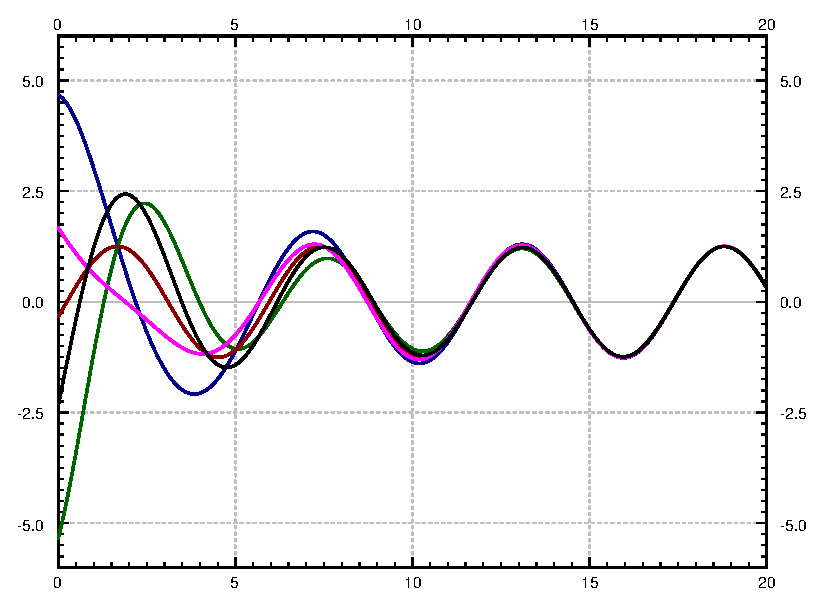
\includegraphics[width=2.5in]{../figures/3-6-transbeh}

\hfill $k=1$, $m=1$, $F_0 = 1$, $c=0.7$, and $\omega=1.1$.

\pause
\vspace*{-1.40in}

The larger the $p$ (that is, $c$), the
faster $x_{tr} \to 0$,

\thus
\quad 
smaller ``transient region.''

\medskip
\pause

$x_{sp}$ is not affected by initial conditions.

\medskip
\pause

\textbf{Remark:}
Undamped motion, $c=0$, means


``infinite transient region''
(i.e., not ``transient'')

\medskip
\pause

We focus on $x_{sp}$ and its amplitude $C$.

\end{frame}

\begin{frame}
There is no (pure) resonance as there is no factor of $t$ in
\[
x_{sp} = 
\frac{F_0}{m \sqrt{{(2\omega p)}^2+{(\omega_0^2-\omega^2)}^2}} 
\cos ( \omega t - \gamma ) .
\]
\pause
We focus on the amplitude as we vary the forcing frequency $\omega$:

\medskip

~~
$\displaystyle
C = C(\omega) =
\frac{F_0}{m \sqrt{{(2\omega p)}^2+{(\omega_0^2-\omega^2)}^2}} 
$
\pause
\vspace*{-0.5in}

\hfill
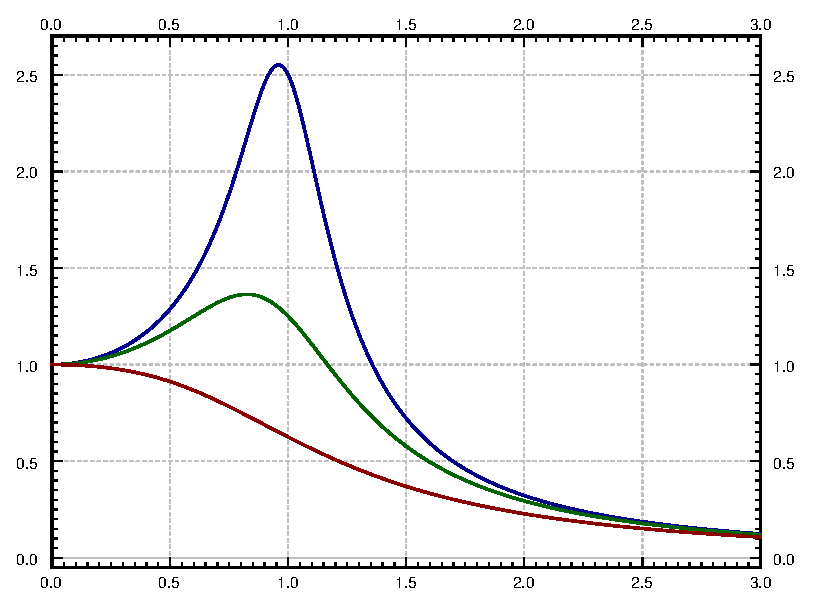
\includegraphics[width=2.5in]{../figures/3-6-pracres}

\vspace*{-1.3in}

Graph of $C(\omega)$ with $k=1$, $m=1$, $F_0 = 1$:

Top line: $c=0.4$, \quad
middle line: $c=0.8$,

bottom line: $c=1.6$.

\medskip
\pause

Call the $\omega > 0$ that maximizes $C$ the

\emph{practical resonance frequency}.

\medskip
\pause

$C(\omega)$ is then the
\emph{practical resonance amplitude}.

\medskip
\pause

We call this \emph{practical resonance}.

\medskip

Practical resonance gets bigger if $c$ gets smaller,
and disappears when damping is too large.
\end{frame}

\begin{frame}

\hfill
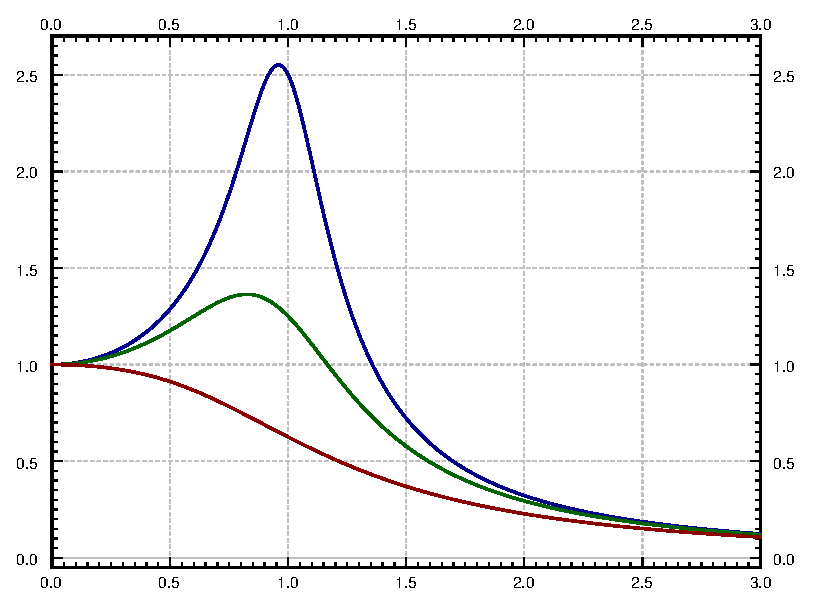
\includegraphics[width=2.1in]{../figures/3-6-pracres}

\vspace*{-1.5in}
To find the max of
\quad
$\displaystyle
C(\omega) =
\frac{F_0}{m \sqrt{{(2\omega p)}^2+{(\omega_0^2-\omega^2)}^2}} ,
$

\medskip

find where
\quad
$\displaystyle
0 =
C'(\omega) =
\frac{- 2\omega( 2p^2+\omega^2-\omega_0^2)F_0}
{m {\bigl({(2\omega p)}^2+{(\omega_0^2-\omega^2)}^2\bigr)}^{3/2}} .
$

\medskip

$C'(\omega) = 0$ when
$\omega = 0$ or
$2p^2+\omega^2-\omega_0^2 = 0$.

\medskip
\pause

At most one critical point for $\omega > 0$.

\medskip
\pause

So there is practical resonance if $2p^2+\omega^2-\omega_0^2 = 0$
has a solution (if $\omega_0^2 - 2p^2 > 0$):
\[
\text{practical resonance }
\omega = \sqrt{\omega_0^2 - 2p^2} .
\]
\pause
If practical resonance occurs, it is smaller than $\omega_0$.

\pause
For very small damping $c$, practical resonance frequency $\omega \approx \omega_0$.

(Indeed, if $c=0$, $\omega_0$ is the (pure) resonance frequency.)

\pause
As $c$ grows, practical resonance frequency $\omega$ goes to $0$.

\medskip
\pause

\textbf{Remark:} $C(\omega) \to 0$ as
$\omega \to \infty$.
\quad\thus\quad
Large forcing frequency means small amplitude.
\end{frame}

\end{document}
